\subsection{Conjuntos de Cantor}

\begin{frame}
\vspace{5pt}
\frametitle{Família Quadrática: Conjuntos de Cantor}
\begin{columns}
\column{\dimexpr\paperwidth-15pt}

Suponha $\mu > 4$. Observe que existem pontos em $[0, 1]$ que não permanecem em $[0, 1]$ após uma iteração de $h$ e, portanto, eles pertencem ao conjunto estável do infinito.

Desse modo, considerando os conjuntos
$$\Lambda_n = \lbrace x \in [0, 1] : h^n(x) \in [0, 1] \rbrace$$ e
$$\Lambda =  \bigcap_{n = 1}^\infty \Lambda_n,$$
podemos estudar a dinâmica de $h: \Lambda \to \Lambda$.

\end{columns}
\end{frame}

%--------------------

\begin{frame}
\frametitle{Família Quadrática: Conjuntos de Cantor}
\begin{columns}
\column{\dimexpr\paperwidth-15pt}

\begin{proposition}
Se $\mu > 4$, então
\begin{enumerate}
\item $\Lambda_n$ é a união de $2^n$ intervalos fechados disjuntos.
\item $h^n: [a, b] \to [0, 1]$ é bijetora, onde $[a, b]$ é um dos intervalos que formam $\Lambda_n$.
\end{enumerate}
\end{proposition}

\begin{figure}[!htb]
\centering
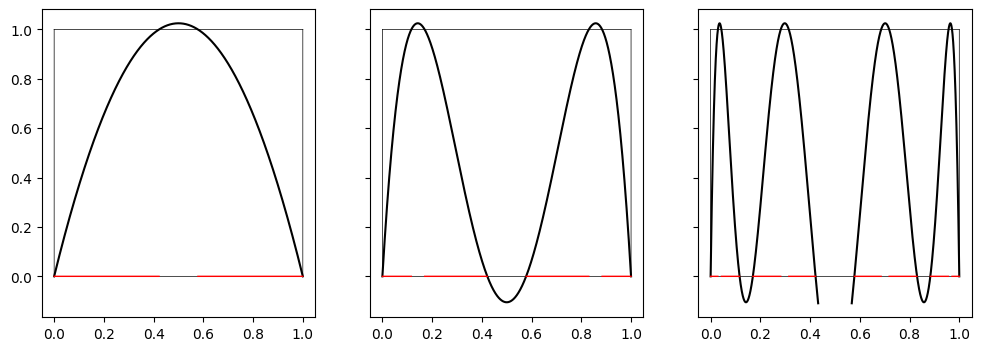
\includegraphics[scale=0.4]{images/h_4,1.png}
\caption{Gráficos de $h$, $h^2$ e $h^3$ para $\mu = 4.1$.}
\label{h_3,839}
\end{figure}

\end{columns}
\end{frame}

%--------------------

\begin{frame}
\vspace{5pt}
\frametitle{Família Quadrática: \subsecname}
\begin{columns}
\column{\dimexpr\paperwidth-15pt}

\begin{lemma}
Se $\mu > 2 + \sqrt{5}$, então
\begin{enumerate}
\item  $|D h(\Lambda_1)| > \lambda > 1$.
\item $b - a < \frac{1}{\lambda^n}$, onde $[a, b]$ é um dos intervalos que formam $\Lambda_n$.
\end{enumerate}
\end{lemma}

\end{columns}
\end{frame}

%--------------------

\begin{frame}
\vspace{5pt}
\frametitle{Família Quadrática: \subsecname}
\begin{columns}
\column{\dimexpr\paperwidth-15pt}

\begin{theorem}
Se $\mu > 2 + \sqrt{5}$, então $\Lambda$ é um conjunto de Cantor \footnote{$\Lambda$ é não vazio, limitado, totalmente desconexo e perfeito.\\}.
\end{theorem}

\begin{proof}
\begin{enumerate}[a)]
\item \textit{$\Lambda$ é totalmente desconexo.}

Se existe $[a, b] \subset \Lambda$, seja $k$ tal que $\frac{1}{\lambda^k} < |a - b|$.
Em particular, $[a, b] \subset \Lambda_k$, o que é um absurdo pois os intervalos que formam $\Lambda_k$ possuem tamanho menor que $\frac{1}{\lambda^k}$.

\item \textit{$\Lambda$ é perfeito.}

Sejam $x \in \Lambda$, $\varepsilon > 0$ e $k \geq 1$ tal que $\frac{1}{\lambda^k} < \varepsilon$.
Se $x \in [a, b]$, onde $[a, b]$ é um dos intervalos que formam $\Lambda_k$, então $a \in \Lambda$ e $|x - a| < \varepsilon$ e, portanto, $x$ é ponto de acumulação de $\Lambda$.
\qedhere
\end{enumerate}
\end{proof}

\begin{block}{Observação}
Esse teorema é válido para $4 < \mu < 2 + \sqrt{5}$, porém a demonstração é mais complicada.
\end{block}

\end{columns}
\end{frame}
